\chapter{A \PD Primer}

\SBGNPDLone is a visual language. Like any language like English it has a vocabulary, which in the case of SBGN is represented by the symbols that we call glyphs. Again like English our language has grammar, which are the underlying rules and concepts of the language that define its meaning. This specification aims to provide a detailed description of both the vocabulary and grammar rules of the language as a reference. However, to understand this it is essential to grasp what an \PDm describes.

The first thing to understand is the SBGN-PD does not describe biochemical reactions or gene expression --- at least not directly. Instead this language describes collections --- pools --- of entities that are manipulated by processes which can convert them from one type of entity to another. An entity pool that is the input to a process is said to consumed and that which is an output is produced. There is a third class of entity pool associated with a process: namely those that affect --- modulate --- the rate at which a process converts entity from one set of pools to another. The amount of entity in a modulating pools is not changed by the process. These very briefly are the key concepts of PD and are illustrated in figure \ref{fig:keyconcepts}.

\begin{figure}[htb]
\begin{center}
\scalebox{0.5}{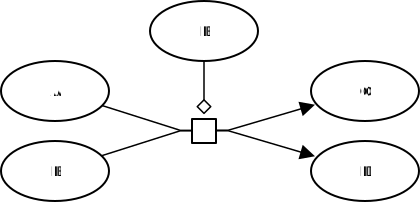
\includegraphics{images/keyconcepts}}
\caption{A process consuming the entity pools A and B and producing the entity pools C and D. The entity pool E modulates the process. The process is represented as a square. Each (unspecified) entity pool is represented as an ellipsis identified by a label. The relationships between the process and each entity pool involved are represented by connecting lines called arcs. Depending on the type of relationship (consumption, production, modulation), these arcs are decorated with different symbols (respectively nothing, arrowhead, and diamond).}\label{fig:key concepts}
\end{center}
\end{figure}

So how do this enable us to describe biological processes? Very simply. Figure \ref{fig:biochem} illustrates a biochemical reaction and shows how the essential components of that reaction, substrate, product and enzyme catalyst are all conveniently described by the representation. Likewise in figure \ref{fig:genereg} we can see again the concept of entity pools and process flow can be applied to gene regulation. This approach gives us a lot of flexibility and enables one to summarise biological processes that may incorporate many biochemical reactions (figure \ref{fig:summarisingproc}).


%%% Diff EPN & Process types here.

In the above examples of biological processes a number of different glyphs where used to illustrate different biological entities: the macromolecule, the simple chemical and the gene.


%%% Compartments.


%%% Clone markers and identity

%%% Logic gates

%%% Maps & Submaps


%%%Overview of the UML/Class specification. 